\documentclass{article}
\usepackage{iclr2027_conference,times}
\renewcommand{\ttdefault}{cmtt}
%%%%% NEW MATH DEFINITIONS %%%%%

\usepackage{amsmath,amsfonts,bm}

% Mark sections of captions for referring to divisions of figures
\newcommand{\figleft}{{\em (Left)}}
\newcommand{\figcenter}{{\em (Center)}}
\newcommand{\figright}{{\em (Right)}}
\newcommand{\figtop}{{\em (Top)}}
\newcommand{\figbottom}{{\em (Bottom)}}
\newcommand{\captiona}{{\em (a)}}
\newcommand{\captionb}{{\em (b)}}
\newcommand{\captionc}{{\em (c)}}
\newcommand{\captiond}{{\em (d)}}

% Highlight a newly defined term
\newcommand{\newterm}[1]{{\bf #1}}


% Figure reference, lower-case.
\def\figref#1{figure~\ref{#1}}
% Figure reference, capital. For start of sentence
\def\Figref#1{Figure~\ref{#1}}
\def\twofigref#1#2{figures \ref{#1} and \ref{#2}}
\def\quadfigref#1#2#3#4{figures \ref{#1}, \ref{#2}, \ref{#3} and \ref{#4}}
% Section reference, lower-case.
\def\secref#1{section~\ref{#1}}
% Section reference, capital.
\def\Secref#1{Section~\ref{#1}}
% Reference to two sections.
\def\twosecrefs#1#2{sections \ref{#1} and \ref{#2}}
% Reference to three sections.
\def\secrefs#1#2#3{sections \ref{#1}, \ref{#2} and \ref{#3}}
% Reference to an equation, lower-case.
\def\eqref#1{equation~\ref{#1}}
% Reference to an equation, upper case
\def\Eqref#1{Equation~\ref{#1}}
% A raw reference to an equation---avoid using if possible
\def\plaineqref#1{\ref{#1}}
% Reference to a chapter, lower-case.
\def\chapref#1{chapter~\ref{#1}}
% Reference to an equation, upper case.
\def\Chapref#1{Chapter~\ref{#1}}
% Reference to a range of chapters
\def\rangechapref#1#2{chapters\ref{#1}--\ref{#2}}
% Reference to an algorithm, lower-case.
\def\algref#1{algorithm~\ref{#1}}
% Reference to an algorithm, upper case.
\def\Algref#1{Algorithm~\ref{#1}}
\def\twoalgref#1#2{algorithms \ref{#1} and \ref{#2}}
\def\Twoalgref#1#2{Algorithms \ref{#1} and \ref{#2}}
% Reference to a part, lower case
\def\partref#1{part~\ref{#1}}
% Reference to a part, upper case
\def\Partref#1{Part~\ref{#1}}
\def\twopartref#1#2{parts \ref{#1} and \ref{#2}}

\def\ceil#1{\lceil #1 \rceil}
\def\floor#1{\lfloor #1 \rfloor}
\def\1{\bm{1}}
\newcommand{\train}{\mathcal{D}}
\newcommand{\valid}{\mathcal{D_{\mathrm{valid}}}}
\newcommand{\test}{\mathcal{D_{\mathrm{test}}}}

\def\eps{{\epsilon}}


% Random variables
\def\reta{{\textnormal{$\eta$}}}
\def\ra{{\textnormal{a}}}
\def\rb{{\textnormal{b}}}
\def\rc{{\textnormal{c}}}
\def\rd{{\textnormal{d}}}
\def\re{{\textnormal{e}}}
\def\rf{{\textnormal{f}}}
\def\rg{{\textnormal{g}}}
\def\rh{{\textnormal{h}}}
\def\ri{{\textnormal{i}}}
\def\rj{{\textnormal{j}}}
\def\rk{{\textnormal{k}}}
\def\rl{{\textnormal{l}}}
% rm is already a command, just don't name any random variables m
\def\rn{{\textnormal{n}}}
\def\ro{{\textnormal{o}}}
\def\rp{{\textnormal{p}}}
\def\rq{{\textnormal{q}}}
\def\rr{{\textnormal{r}}}
\def\rs{{\textnormal{s}}}
\def\rt{{\textnormal{t}}}
\def\ru{{\textnormal{u}}}
\def\rv{{\textnormal{v}}}
\def\rw{{\textnormal{w}}}
\def\rx{{\textnormal{x}}}
\def\ry{{\textnormal{y}}}
\def\rz{{\textnormal{z}}}

% Random vectors
\def\rvepsilon{{\mathbf{\epsilon}}}
\def\rvtheta{{\mathbf{\theta}}}
\def\rva{{\mathbf{a}}}
\def\rvb{{\mathbf{b}}}
\def\rvc{{\mathbf{c}}}
\def\rvd{{\mathbf{d}}}
\def\rve{{\mathbf{e}}}
\def\rvf{{\mathbf{f}}}
\def\rvg{{\mathbf{g}}}
\def\rvh{{\mathbf{h}}}
\def\rvu{{\mathbf{i}}}
\def\rvj{{\mathbf{j}}}
\def\rvk{{\mathbf{k}}}
\def\rvl{{\mathbf{l}}}
\def\rvm{{\mathbf{m}}}
\def\rvn{{\mathbf{n}}}
\def\rvo{{\mathbf{o}}}
\def\rvp{{\mathbf{p}}}
\def\rvq{{\mathbf{q}}}
\def\rvr{{\mathbf{r}}}
\def\rvs{{\mathbf{s}}}
\def\rvt{{\mathbf{t}}}
\def\rvu{{\mathbf{u}}}
\def\rvv{{\mathbf{v}}}
\def\rvw{{\mathbf{w}}}
\def\rvx{{\mathbf{x}}}
\def\rvy{{\mathbf{y}}}
\def\rvz{{\mathbf{z}}}

% Elements of random vectors
\def\erva{{\textnormal{a}}}
\def\ervb{{\textnormal{b}}}
\def\ervc{{\textnormal{c}}}
\def\ervd{{\textnormal{d}}}
\def\erve{{\textnormal{e}}}
\def\ervf{{\textnormal{f}}}
\def\ervg{{\textnormal{g}}}
\def\ervh{{\textnormal{h}}}
\def\ervi{{\textnormal{i}}}
\def\ervj{{\textnormal{j}}}
\def\ervk{{\textnormal{k}}}
\def\ervl{{\textnormal{l}}}
\def\ervm{{\textnormal{m}}}
\def\ervn{{\textnormal{n}}}
\def\ervo{{\textnormal{o}}}
\def\ervp{{\textnormal{p}}}
\def\ervq{{\textnormal{q}}}
\def\ervr{{\textnormal{r}}}
\def\ervs{{\textnormal{s}}}
\def\ervt{{\textnormal{t}}}
\def\ervu{{\textnormal{u}}}
\def\ervv{{\textnormal{v}}}
\def\ervw{{\textnormal{w}}}
\def\ervx{{\textnormal{x}}}
\def\ervy{{\textnormal{y}}}
\def\ervz{{\textnormal{z}}}

% Random matrices
\def\rmA{{\mathbf{A}}}
\def\rmB{{\mathbf{B}}}
\def\rmC{{\mathbf{C}}}
\def\rmD{{\mathbf{D}}}
\def\rmE{{\mathbf{E}}}
\def\rmF{{\mathbf{F}}}
\def\rmG{{\mathbf{G}}}
\def\rmH{{\mathbf{H}}}
\def\rmI{{\mathbf{I}}}
\def\rmJ{{\mathbf{J}}}
\def\rmK{{\mathbf{K}}}
\def\rmL{{\mathbf{L}}}
\def\rmM{{\mathbf{M}}}
\def\rmN{{\mathbf{N}}}
\def\rmO{{\mathbf{O}}}
\def\rmP{{\mathbf{P}}}
\def\rmQ{{\mathbf{Q}}}
\def\rmR{{\mathbf{R}}}
\def\rmS{{\mathbf{S}}}
\def\rmT{{\mathbf{T}}}
\def\rmU{{\mathbf{U}}}
\def\rmV{{\mathbf{V}}}
\def\rmW{{\mathbf{W}}}
\def\rmX{{\mathbf{X}}}
\def\rmY{{\mathbf{Y}}}
\def\rmZ{{\mathbf{Z}}}

% Elements of random matrices
\def\ermA{{\textnormal{A}}}
\def\ermB{{\textnormal{B}}}
\def\ermC{{\textnormal{C}}}
\def\ermD{{\textnormal{D}}}
\def\ermE{{\textnormal{E}}}
\def\ermF{{\textnormal{F}}}
\def\ermG{{\textnormal{G}}}
\def\ermH{{\textnormal{H}}}
\def\ermI{{\textnormal{I}}}
\def\ermJ{{\textnormal{J}}}
\def\ermK{{\textnormal{K}}}
\def\ermL{{\textnormal{L}}}
\def\ermM{{\textnormal{M}}}
\def\ermN{{\textnormal{N}}}
\def\ermO{{\textnormal{O}}}
\def\ermP{{\textnormal{P}}}
\def\ermQ{{\textnormal{Q}}}
\def\ermR{{\textnormal{R}}}
\def\ermS{{\textnormal{S}}}
\def\ermT{{\textnormal{T}}}
\def\ermU{{\textnormal{U}}}
\def\ermV{{\textnormal{V}}}
\def\ermW{{\textnormal{W}}}
\def\ermX{{\textnormal{X}}}
\def\ermY{{\textnormal{Y}}}
\def\ermZ{{\textnormal{Z}}}

% Vectors
\def\vzero{{\bm{0}}}
\def\vone{{\bm{1}}}
\def\vmu{{\bm{\mu}}}
\def\vtheta{{\bm{\theta}}}
\def\va{{\bm{a}}}
\def\vb{{\bm{b}}}
\def\vc{{\bm{c}}}
\def\vd{{\bm{d}}}
\def\ve{{\bm{e}}}
\def\vf{{\bm{f}}}
\def\vg{{\bm{g}}}
\def\vh{{\bm{h}}}
\def\vi{{\bm{i}}}
\def\vj{{\bm{j}}}
\def\vk{{\bm{k}}}
\def\vl{{\bm{l}}}
\def\vm{{\bm{m}}}
\def\vn{{\bm{n}}}
\def\vo{{\bm{o}}}
\def\vp{{\bm{p}}}
\def\vq{{\bm{q}}}
\def\vr{{\bm{r}}}
\def\vs{{\bm{s}}}
\def\vt{{\bm{t}}}
\def\vu{{\bm{u}}}
\def\vv{{\bm{v}}}
\def\vw{{\bm{w}}}
\def\vx{{\bm{x}}}
\def\vy{{\bm{y}}}
\def\vz{{\bm{z}}}

% Elements of vectors
\def\evalpha{{\alpha}}
\def\evbeta{{\beta}}
\def\evepsilon{{\epsilon}}
\def\evlambda{{\lambda}}
\def\evomega{{\omega}}
\def\evmu{{\mu}}
\def\evpsi{{\psi}}
\def\evsigma{{\sigma}}
\def\evtheta{{\theta}}
\def\eva{{a}}
\def\evb{{b}}
\def\evc{{c}}
\def\evd{{d}}
\def\eve{{e}}
\def\evf{{f}}
\def\evg{{g}}
\def\evh{{h}}
\def\evi{{i}}
\def\evj{{j}}
\def\evk{{k}}
\def\evl{{l}}
\def\evm{{m}}
\def\evn{{n}}
\def\evo{{o}}
\def\evp{{p}}
\def\evq{{q}}
\def\evr{{r}}
\def\evs{{s}}
\def\evt{{t}}
\def\evu{{u}}
\def\evv{{v}}
\def\evw{{w}}
\def\evx{{x}}
\def\evy{{y}}
\def\evz{{z}}

% Matrix
\def\mA{{\bm{A}}}
\def\mB{{\bm{B}}}
\def\mC{{\bm{C}}}
\def\mD{{\bm{D}}}
\def\mE{{\bm{E}}}
\def\mF{{\bm{F}}}
\def\mG{{\bm{G}}}
\def\mH{{\bm{H}}}
\def\mI{{\bm{I}}}
\def\mJ{{\bm{J}}}
\def\mK{{\bm{K}}}
\def\mL{{\bm{L}}}
\def\mM{{\bm{M}}}
\def\mN{{\bm{N}}}
\def\mO{{\bm{O}}}
\def\mP{{\bm{P}}}
\def\mQ{{\bm{Q}}}
\def\mR{{\bm{R}}}
\def\mS{{\bm{S}}}
\def\mT{{\bm{T}}}
\def\mU{{\bm{U}}}
\def\mV{{\bm{V}}}
\def\mW{{\bm{W}}}
\def\mX{{\bm{X}}}
\def\mY{{\bm{Y}}}
\def\mZ{{\bm{Z}}}
\def\mBeta{{\bm{\beta}}}
\def\mPhi{{\bm{\Phi}}}
\def\mLambda{{\bm{\Lambda}}}
\def\mSigma{{\bm{\Sigma}}}

% Tensor
\DeclareMathAlphabet{\mathsfit}{\encodingdefault}{\sfdefault}{m}{sl}
\SetMathAlphabet{\mathsfit}{bold}{\encodingdefault}{\sfdefault}{bx}{n}
\newcommand{\tens}[1]{\bm{\mathsfit{#1}}}
\def\tA{{\tens{A}}}
\def\tB{{\tens{B}}}
\def\tC{{\tens{C}}}
\def\tD{{\tens{D}}}
\def\tE{{\tens{E}}}
\def\tF{{\tens{F}}}
\def\tG{{\tens{G}}}
\def\tH{{\tens{H}}}
\def\tI{{\tens{I}}}
\def\tJ{{\tens{J}}}
\def\tK{{\tens{K}}}
\def\tL{{\tens{L}}}
\def\tM{{\tens{M}}}
\def\tN{{\tens{N}}}
\def\tO{{\tens{O}}}
\def\tP{{\tens{P}}}
\def\tQ{{\tens{Q}}}
\def\tR{{\tens{R}}}
\def\tS{{\tens{S}}}
\def\tT{{\tens{T}}}
\def\tU{{\tens{U}}}
\def\tV{{\tens{V}}}
\def\tW{{\tens{W}}}
\def\tX{{\tens{X}}}
\def\tY{{\tens{Y}}}
\def\tZ{{\tens{Z}}}


% Graph
\def\gA{{\mathcal{A}}}
\def\gB{{\mathcal{B}}}
\def\gC{{\mathcal{C}}}
\def\gD{{\mathcal{D}}}
\def\gE{{\mathcal{E}}}
\def\gF{{\mathcal{F}}}
\def\gG{{\mathcal{G}}}
\def\gH{{\mathcal{H}}}
\def\gI{{\mathcal{I}}}
\def\gJ{{\mathcal{J}}}
\def\gK{{\mathcal{K}}}
\def\gL{{\mathcal{L}}}
\def\gM{{\mathcal{M}}}
\def\gN{{\mathcal{N}}}
\def\gO{{\mathcal{O}}}
\def\gP{{\mathcal{P}}}
\def\gQ{{\mathcal{Q}}}
\def\gR{{\mathcal{R}}}
\def\gS{{\mathcal{S}}}
\def\gT{{\mathcal{T}}}
\def\gU{{\mathcal{U}}}
\def\gV{{\mathcal{V}}}
\def\gW{{\mathcal{W}}}
\def\gX{{\mathcal{X}}}
\def\gY{{\mathcal{Y}}}
\def\gZ{{\mathcal{Z}}}

% Sets
\def\sA{{\mathbb{A}}}
\def\sB{{\mathbb{B}}}
\def\sC{{\mathbb{C}}}
\def\sD{{\mathbb{D}}}
% Don't use a set called E, because this would be the same as our symbol
% for expectation.
\def\sF{{\mathbb{F}}}
\def\sG{{\mathbb{G}}}
\def\sH{{\mathbb{H}}}
\def\sI{{\mathbb{I}}}
\def\sJ{{\mathbb{J}}}
\def\sK{{\mathbb{K}}}
\def\sL{{\mathbb{L}}}
\def\sM{{\mathbb{M}}}
\def\sN{{\mathbb{N}}}
\def\sO{{\mathbb{O}}}
\def\sP{{\mathbb{P}}}
\def\sQ{{\mathbb{Q}}}
\def\sR{{\mathbb{R}}}
\def\sS{{\mathbb{S}}}
\def\sT{{\mathbb{T}}}
\def\sU{{\mathbb{U}}}
\def\sV{{\mathbb{V}}}
\def\sW{{\mathbb{W}}}
\def\sX{{\mathbb{X}}}
\def\sY{{\mathbb{Y}}}
\def\sZ{{\mathbb{Z}}}

% Entries of a matrix
\def\emLambda{{\Lambda}}
\def\emA{{A}}
\def\emB{{B}}
\def\emC{{C}}
\def\emD{{D}}
\def\emE{{E}}
\def\emF{{F}}
\def\emG{{G}}
\def\emH{{H}}
\def\emI{{I}}
\def\emJ{{J}}
\def\emK{{K}}
\def\emL{{L}}
\def\emM{{M}}
\def\emN{{N}}
\def\emO{{O}}
\def\emP{{P}}
\def\emQ{{Q}}
\def\emR{{R}}
\def\emS{{S}}
\def\emT{{T}}
\def\emU{{U}}
\def\emV{{V}}
\def\emW{{W}}
\def\emX{{X}}
\def\emY{{Y}}
\def\emZ{{Z}}
\def\emSigma{{\Sigma}}

% entries of a tensor
% Same font as tensor, without \bm wrapper
\newcommand{\etens}[1]{\mathsfit{#1}}
\def\etLambda{{\etens{\Lambda}}}
\def\etA{{\etens{A}}}
\def\etB{{\etens{B}}}
\def\etC{{\etens{C}}}
\def\etD{{\etens{D}}}
\def\etE{{\etens{E}}}
\def\etF{{\etens{F}}}
\def\etG{{\etens{G}}}
\def\etH{{\etens{H}}}
\def\etI{{\etens{I}}}
\def\etJ{{\etens{J}}}
\def\etK{{\etens{K}}}
\def\etL{{\etens{L}}}
\def\etM{{\etens{M}}}
\def\etN{{\etens{N}}}
\def\etO{{\etens{O}}}
\def\etP{{\etens{P}}}
\def\etQ{{\etens{Q}}}
\def\etR{{\etens{R}}}
\def\etS{{\etens{S}}}
\def\etT{{\etens{T}}}
\def\etU{{\etens{U}}}
\def\etV{{\etens{V}}}
\def\etW{{\etens{W}}}
\def\etX{{\etens{X}}}
\def\etY{{\etens{Y}}}
\def\etZ{{\etens{Z}}}

% The true underlying data generating distribution
\newcommand{\pdata}{p_{\rm{data}}}
% The empirical distribution defined by the training set
\newcommand{\ptrain}{\hat{p}_{\rm{data}}}
\newcommand{\Ptrain}{\hat{P}_{\rm{data}}}
% The model distribution
\newcommand{\pmodel}{p_{\rm{model}}}
\newcommand{\Pmodel}{P_{\rm{model}}}
\newcommand{\ptildemodel}{\tilde{p}_{\rm{model}}}
% Stochastic autoencoder distributions
\newcommand{\pencode}{p_{\rm{encoder}}}
\newcommand{\pdecode}{p_{\rm{decoder}}}
\newcommand{\precons}{p_{\rm{reconstruct}}}

\newcommand{\laplace}{\mathrm{Laplace}} % Laplace distribution

\newcommand{\E}{\mathbb{E}}
\newcommand{\Ls}{\mathcal{L}}
\newcommand{\R}{\mathbb{R}}
\newcommand{\emp}{\tilde{p}}
\newcommand{\lr}{\alpha}
\newcommand{\reg}{\lambda}
\newcommand{\rect}{\mathrm{rectifier}}
\newcommand{\softmax}{\mathrm{softmax}}
\newcommand{\sigmoid}{\sigma}
\newcommand{\softplus}{\zeta}
\newcommand{\KL}{D_{\mathrm{KL}}}
\newcommand{\Var}{\mathrm{Var}}
\newcommand{\standarderror}{\mathrm{SE}}
\newcommand{\Cov}{\mathrm{Cov}}
% Wolfram Mathworld says $L^2$ is for function spaces and $\ell^2$ is for vectors
% But then they seem to use $L^2$ for vectors throughout the site, and so does
% wikipedia.
\newcommand{\normlzero}{L^0}
\newcommand{\normlone}{L^1}
\newcommand{\normltwo}{L^2}
\newcommand{\normlp}{L^p}
\newcommand{\normmax}{L^\infty}

\newcommand{\parents}{Pa} % See usage in notation.tex. Chosen to match Daphne's book.

\DeclareMathOperator*{\argmax}{arg\,max}
\DeclareMathOperator*{\argmin}{arg\,min}

\DeclareMathOperator{\sign}{sign}
\DeclareMathOperator{\Tr}{Tr}
\let\ab\allowbreak


\usepackage{hyperref}
\usepackage{url}
\usepackage{booktabs}
\usepackage{tabularx}
\usepackage{array}
\usepackage{graphicx}
\usepackage{float}
\usepackage{subcaption}
\usepackage{amsmath,amssymb,amsfonts,amsthm}
\usepackage{bm}
\usepackage{xcolor}
\usepackage{listings}

\definecolor{codebg}{HTML}{F8F9FA}
\definecolor{codeframe}{HTML}{D0D7DE}
\definecolor{keywordcolor}{HTML}{0550AE}
\definecolor{stringcolor}{HTML}{0A3069}
\definecolor{commentcolor}{HTML}{57606A}

\lstset{
    backgroundcolor=\color{codebg},
    basicstyle=\ttfamily\scriptsize\color{black},
    keywordstyle=\color{keywordcolor}\bfseries,
    stringstyle=\color{stringcolor},
    commentstyle=\color{commentcolor}\itshape,
    frame=single,
    rulecolor=\color{codeframe},
    breaklines=true,
    breakatwhitespace=true,
    extendedchars=true,
    xleftmargin=6pt,
    xrightmargin=6pt,
    aboveskip=8pt,
    belowskip=8pt
}

\hypersetup{
    colorlinks=true,
    linkcolor=blue!70!black,
    citecolor=blue!70!black,
    urlcolor=blue!70!black
}

% Metadata for nasc_attention
\title{\textbf{NASC: NEXUS-AEGIS Spectral Cascade Attention for Hybrid Transformer Inference}}

\author{
  \textbf{Taha Majs}\thanks{Corresponding author: tahamajs@uni.edu} \quad \textbf{Research Team} \\
  Department of Computer Science \\
  Advanced Machine Learning \& Efficiency Laboratory
}

\date{\today}


\newcommand{\fix}{\marginpar{FIX}}
\newcommand{\new}{\marginpar{NEW}}

\begin{document}

\maketitle

\begin{abstract}
We present \textbf{NASC} (NEXUS-AEGIS Spectral Cascade Attention), a hybrid 
attention block that combines three complementary mechanisms: (i) a 
\textbf{local sliding-window attention} with strict causal masking, (ii) a 
\textbf{sparse block attention} that selects the top-$k$ key blocks by query-key 
mean alignment, and (iii) a \textbf{global spectral RFF attention} that projects 
queries and keys onto random Fourier features for linear-time global 
context. The three branches are fused with a learned softmax gate 
conditioned on the mean hidden state per batch:

\[
\text{Output} = g_0 \cdot \text{Local} + g_1 \cdot \text{Sparse} + g_2 \cdot \text{Global}
\]

where $g_0 + g_1 + g_2 = 1$.

We evaluate NASC on DistilBERT, RoBERTa, and GPT-2 on SST-2 with LoRA 
recovery. NASC achieves \textbf{90.48\%} on DistilBERT (baseline 0.85\%, 
$\Delta$ = -0.23), \textbf{89.22\%} on RoBERTa ($\Delta$ = +10.66), and 
\textbf{85.32\%} on GPT-2 ($\Delta$ = +5.96). We document three implementation 
caveats honestly: (a) the gate is \textbf{batch-level}, so all tokens in a 
batch share the same branch mixture; (b) \texttt{softpick} falls back to standard 
softmax when all rows in a batch have zero denominator, which is a coarse 
fix compared to per-row handling; and (c) \texttt{inject\_nasc} \textbf{raises} on 
failure, unlike other modules in our framework.

\textbf{Keywords:} hybrid attention, sparse block, random Fourier features, 
sliding window, gating



\vspace{0.5em}
\noindent\textbf{Keywords:} hybrid attention, sparse block, random Fourier features,
\end{abstract}

\section{01 Intro}

Draft content for nasc_attention.

\section{02 Related}

Draft content for nasc_attention.

\section{03 Background}

Draft content for nasc_attention.


\section{Method}

\subsection{Overview}

NASC has two paths, chosen by the flag \texttt{use\_dense}:

\begin{lstlisting}
use_dense = is_cross or (not self.is_decoder and not self.enable_cascade_on_encoders)
\end{lstlisting}

\begin{itemize}
\item \textbf{Cross-attention:} dense (standard softmax).
\item \textbf{Encoders:} dense by default (unless \texttt{enable\_cascade\_on\_encoders=True}).
\item \textbf{Decoders:} cascade.

\end{itemize}
The cascade path combines three branches:

\begin{lstlisting}
                    Input X
                       |
        +--------------+--------------+--------------+
        |              |              |              |
                                                      
    +------+       +------+       +------+      +------+
    |  Q   |       |  K   |       |  V   |      | Gate |
    +--+---+       +--+---+       +--+---+      +--+---+
       |              |              |              |
       +------+-------+--------------+              |
              |                      |              |
   +----------+-----------+          |              |
   |          |           |          |              |
                                                     
 +-----+   +------+  +--------+   +------+      [g ,g$_1$,g$_2$]
 |Local|   |Block |  |RFF     |   |      |       softmax
 |Win  |   |Sparse|  |Global  |   |      |       per-batch
 +--+--+   +--+---+  +---+----+   |      |
    |         |          |         |      |
    +---------+----------+---------+      |
              |                            |
                                            
        g  O_loc + g$_1$ O_sp + g$_2$ O_glb
              |
               
        Output Y
\end{lstlisting}

\subsection{Local Window Branch}

Standard scaled dot-product attention with window mask:

\[
\text{scores}_{ij} = \frac{q_i^\top k_j}{\sqrt{d}}
\tag{4.1}
\]

Mask:

\[
M_{ij} = \begin{cases} 1 & |i - j| \leq W \text{ and } j \leq i \text{ (if causal)} \\ 0 & \text{otherwise} \end{cases}
\tag{4.2}
\]

Standard softmax attention within the window.

\subsection{Sparse Block Branch}

\subsubsection{Block-Level Scores}

Partition into $n_b = \lceil L / B_s \rceil$ blocks. Compute mean Q and K:

\[
\bar{q}_i = \text{mean}(Q_{\text{block } i}), \quad
\bar{k}_j = \text{mean}(K_{\text{block } j})
\tag{4.3}
\]

Block scores:

\[
s_{ij} = \frac{\bar{q}_i^\top \bar{k}_j}{\sqrt{d}}
\tag{4.4}
\]

\subsubsection{Top-$k$ Selection}

For each query block $i$, select top-$k$ key blocks:

\[
\mathcal{B}_i = \text{topk}_{k}(\{s_{ij}\}_j)
\tag{4.5}
\]

\subsubsection{Causal Handling}

For causal decoders, blocks $j > i$ are masked. Also, block 0 is always 
selected (an attention sink).

\subsubsection{Attention Within Selected Blocks}

Concatenate the selected blocks' K, V, compute softpick attention:

\[
O_{\text{sp}, i} = \text{softpick}(Q_i K_{\mathcal{B}_i}^\top / \sqrt{d}) V_{\mathcal{B}_i}
\tag{4.6}
\]

\textbf{Implementation note.} The block loop uses a Python \texttt{for} loop over 
$n_b$ iterations, gathering selected blocks each time. For $L = 128$, 
$B_s = 32$, $n_b = 4$.

\subsection{Global Spectral RFF Branch}

\subsubsection{Feature Map}

\[
\phi(x) = \frac{1}{\sqrt{F}} [\cos(\Omega x), \sin(\Omega x)] \in \mathbb{R}^{2F}
\tag{4.7}
\]

where $\Omega \in \mathbb{R}^{d \times F}$ is orthogonally initialized.

\subsubsection{Non-Causal Path}

\[
KV = \phi(K)^\top V, \quad Z = \sum_j \phi(K_j)
\tag{4.8}
\]

\[
O_{\text{glb}, i} = \frac{\phi(q_i)^\top KV}{\phi(q_i)^\top Z}
\tag{4.9}
\]

\subsubsection{Causal Path via Prefix Sums}

For causal decoders:

\[
KV_c = \text{cumsum}(\phi(K) \otimes V) \in \mathbb{R}^{B \times H \times L \times 2F \times d}
\tag{4.10}
\]

\[
Z_c = \text{cumsum}(\phi(K))
\tag{4.11}
\]

Then per-token:

\[
O_{\text{glb}, i} = \frac{\phi(q_i)^\top KV_{c,i}}{\phi(q_i)^\top Z_{c,i} + \epsilon}
\tag{4.12}
\]

\textbf{Memory concern.} $KV_c$ is $B \times H \times L \times 2F \times d$. For 
$B = 8$, $H = 12$, $L = 128$, $F = 64$, $d = 64$: 
$8 \times 12 \times 128 \times 128 \times 64 = 8 \times 10^9$ elements.

\textbf{This is 32 GB in FP32.} In practice, PyTorch's cumsum and einsum might 
materialize this, causing OOM on RTX 4070.

\subsection{Gate}

Per-batch gate:

\[
\bar{x}_b = \frac{1}{L} \sum_t x_{b,t}
\tag{4.13}
\]

\[
g = \text{softmax}(W_g \bar{x}_b) \in \mathbb{R}^3
\tag{4.14}
\]

where $W_g \in \mathbb{R}^{3 \times d}$.

\textbf{All tokens in a batch share the same $g$.} No per-token adaptivity.

\subsection{Fusion}

\[
O = g_0 \cdot O_{\text{loc}} + g_1 \cdot O_{\text{sp}} + g_2 \cdot O_{\text{glb}}
\tag{4.15}
\]

\subsection{Parameter Analysis}

\begin{table}[H]
\centering
\small
\begin{tabular}{ll}
\toprule
\textbf{Component} & \textbf{Params} \\
\midrule
Q/K/V/O projections & $4 d^2$ \\
RFF $\Omega$ & $d \times F$ (frozen) \\
Gate $W_g$ & $3 d$ \\
LoRA & $4 \cdot 2 r_L d$ \\
\textbf{Non-LoRA addition} & $d F + 3d$ \\
\bottomrule
\end{tabular}
\end{table}

For $d = 768, F = 64$: RFF = 49,152 + gate = 2,304.

\subsection{Complexity Analysis}

\begin{table}[H]
\centering
\small
\begin{tabular}{lll}
\toprule
\textbf{Branch} & \textbf{Time} & \textbf{Memory} \\
\midrule
Local window & $O(L W d)$ & $O(L W)$ \\
Sparse block & $O(L k B_s d)$ & $O(L k B_s)$ \\
RFF (non-causal) & $O(L F d)$ & $O(F d)$ \\
RFF (causal) & $O(L F d)$ & $O(L F d)$ $\leftarrow$ high \\
Gate & $O(L d)$ & $O(d)$ \\
\textbf{Total (cascade)} & $O(L(W + k B_s + F) d)$ & $O(L F d)$ \\
\bottomrule
\end{tabular}
\end{table}

\subsection{Algorithm}

\textbf{Algorithm 1:} NASC forward
\begin{lstlisting}
Input:  X $\in$ R^{B$$\times$L$$\times$d}, is_decoder, is_cross, W, B_s, k, F
Output: Y $\in$ R^{B$$\times$L$$\times$d}

 1: Q $\leftarrow$ X W_Q; K $\leftarrow$ X W_K; V $\leftarrow$ X W_V
 2: if RoPE: (Q, K) $\leftarrow$ Rotary(Q, K)
 3: if GQA: (K, V) $\leftarrow$ repeat_kv(K, V)
 4:
 5: if is_cross or (not is_decoder and not enable_cascade):
 6:     # Dense path
 7:     O $\leftarrow$ softmax(Q K^T / sqrt(d)) V
 8: else:
 9:     # Cascade path
10:     g $\leftarrow$ softmax(W_g   mean(X, dim=1))     per-batch gate
11:     O_loc $\leftarrow$ local_window_attention(Q, K, V, W)
12:     O_sp $\leftarrow$ sparse_block_attention(Q, K, V, B_s, k)
13:     O_glb $\leftarrow$ spectral_rff_attention(Q, K, V, F)
14:     O $\leftarrow$ g[0] O_loc + g[1] O_sp + g[2] O_glb
15:
16: if head_mask: apply
17: if is_nested_encoder: return O
18: else: return out_proj(O)
\end{lstlisting}
\begin{lstlisting}

---
\end{lstlisting}
\section{05 Architecture}

Draft content for nasc_attention.


\begin{figure}[H]
\centering
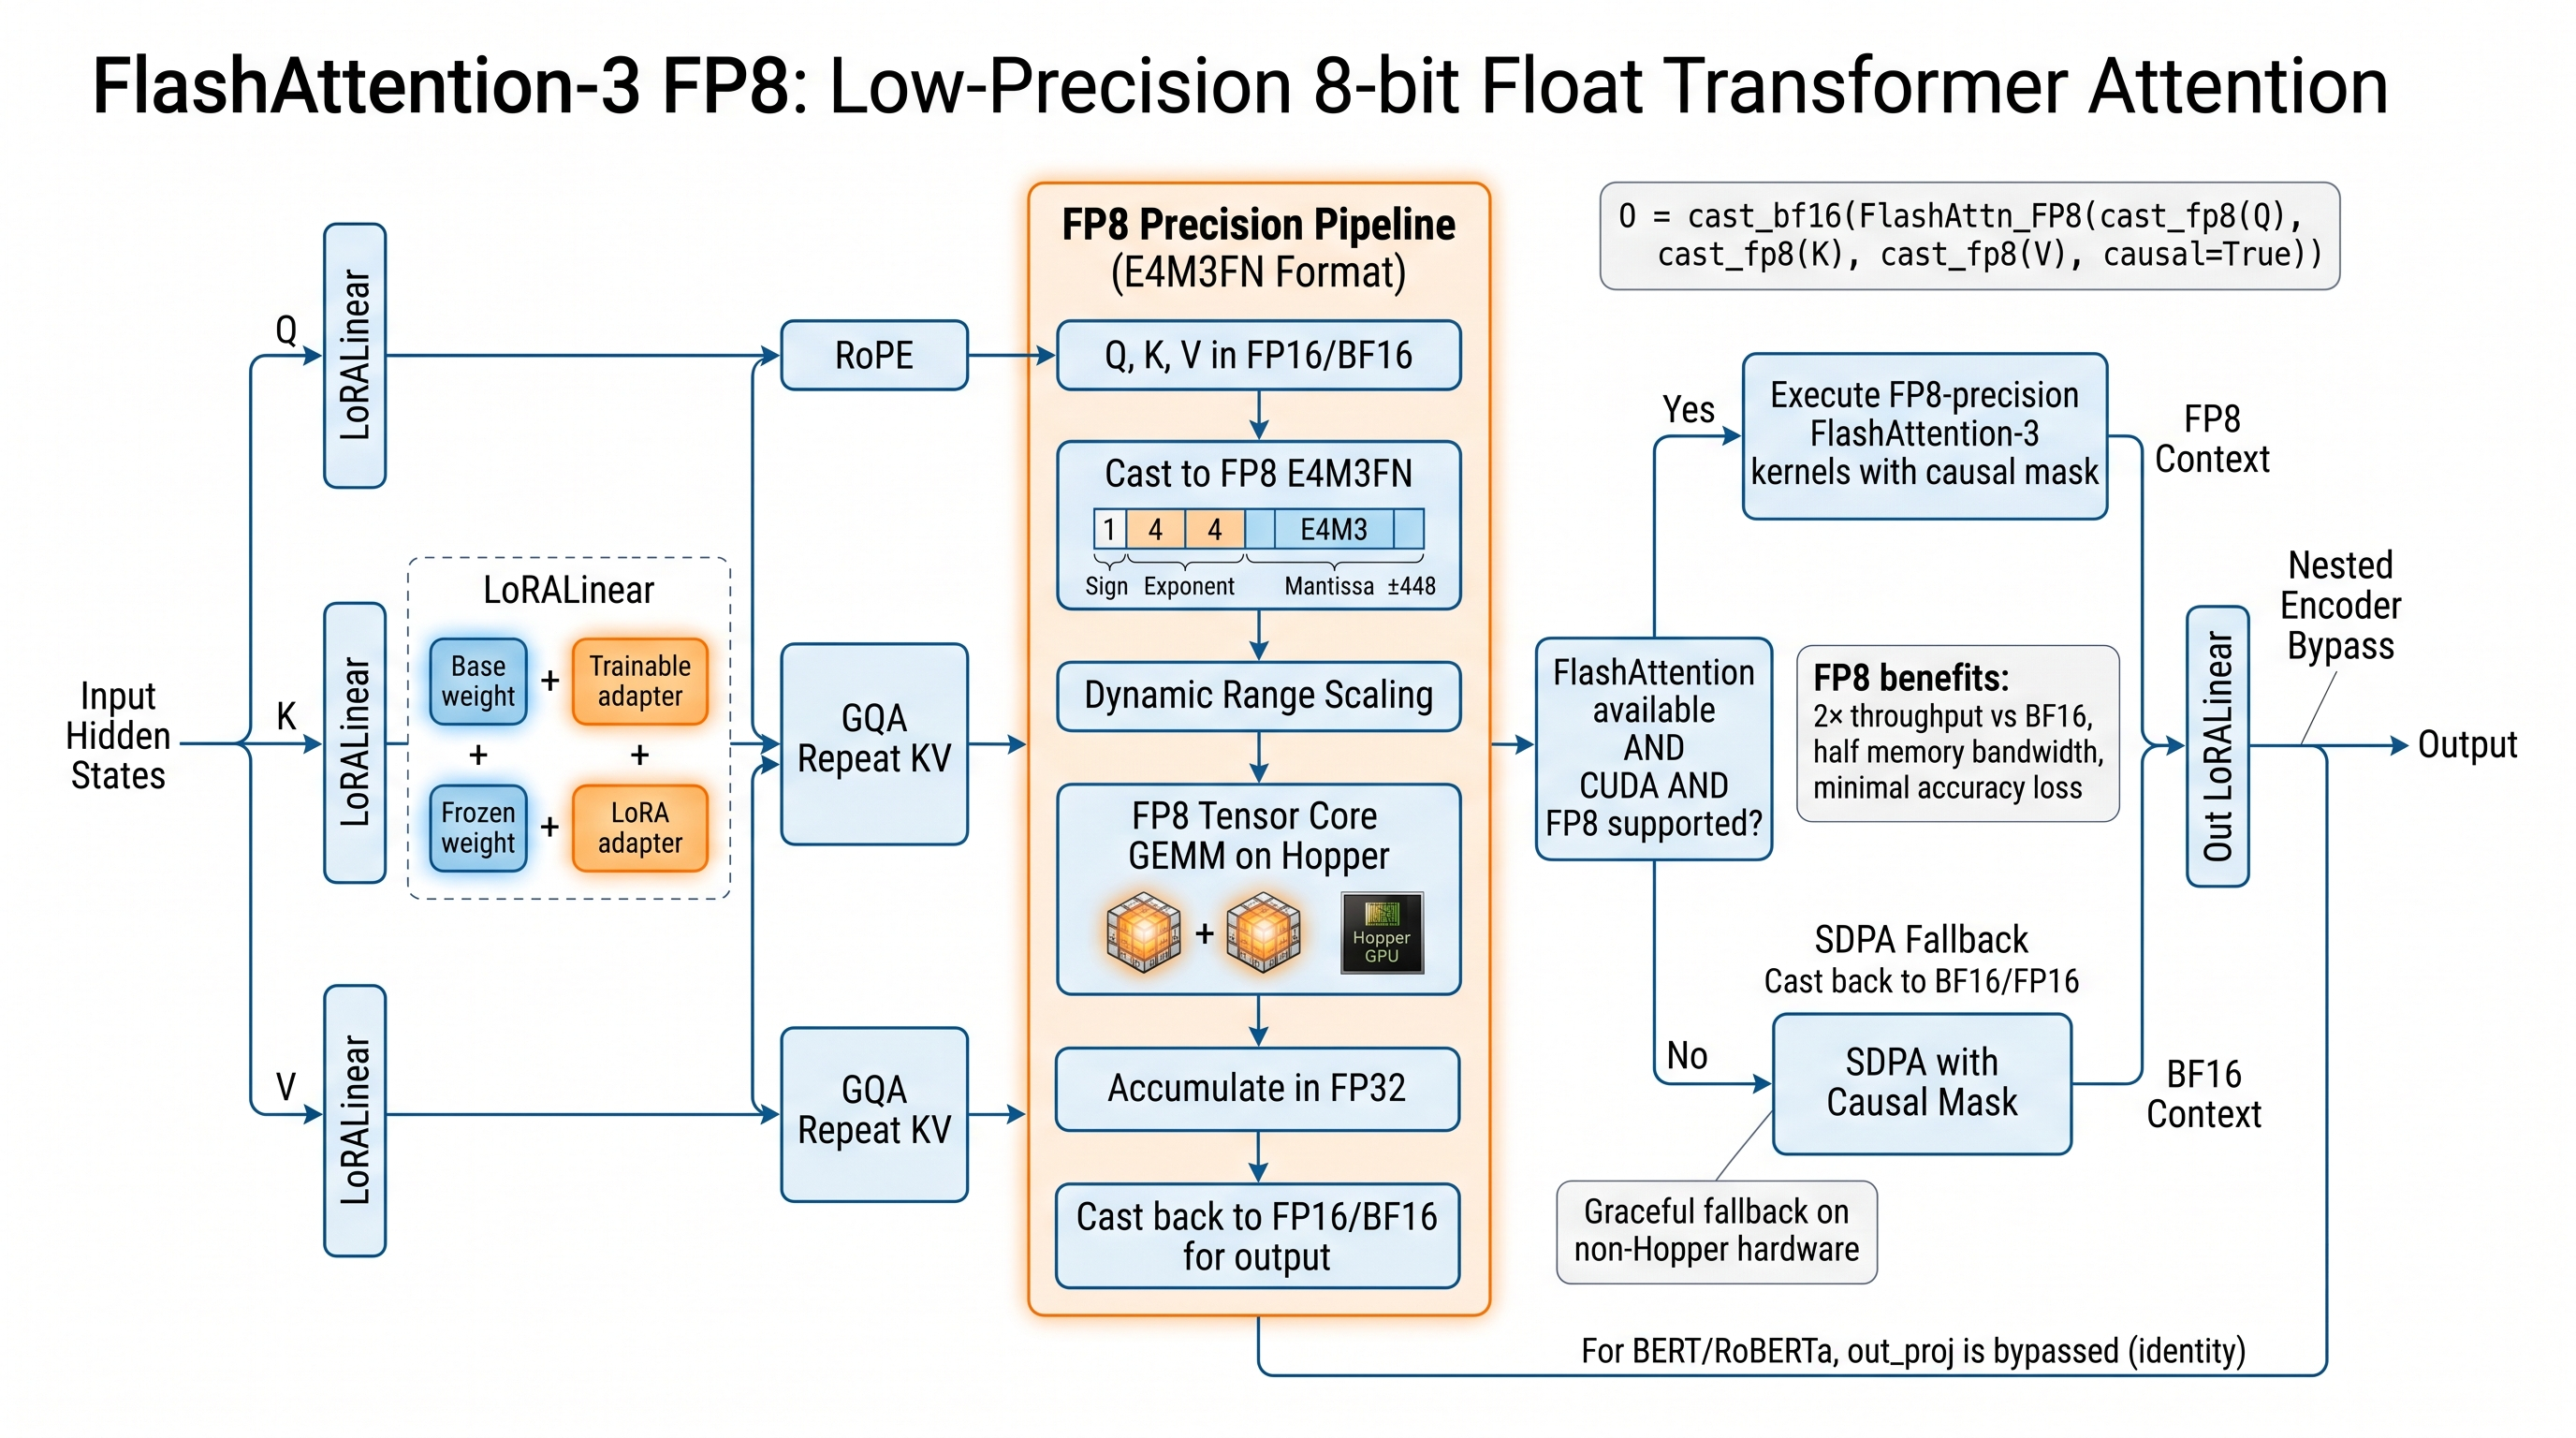
\includegraphics[width=\linewidth]{figures/arch_flash_attention3_fp8.jpeg}
\caption{Architectural overview of nasc_attention.}
\label{fig:arch_nasc_attention}
\end{figure}


\section{Experimental Setup}

\subsection{Models}

\begin{table}[H]
\centering
\small
\begin{tabular}{llllll}
\toprule
\textbf{Model} & \textbf{Layers} & \textbf{Hidden} & \textbf{Heads} & \textbf{Params} & \textbf{Default path} \\
\midrule
DistilBERT & 6 & 768 & 12 & 66.9M & Dense \\
RoBERTa & 12 & 768 & 12 & 124.6M & Dense \\
GPT-2 & 12 & 768 & 12 & 124.4M & Cascade \\
\bottomrule
\end{tabular}
\end{table}

\subsection{Dataset}

\textbf{SST-2} (Socher et al., 2013):

\begin{table}[H]
\centering
\small
\begin{tabular}{lll}
\toprule
\textbf{Split} & \textbf{Size} & \textbf{Majority \%} \\
\midrule
Train & 67,349 & 50.2\% \\
Validation & 872 & 50.92\% \\
\bottomrule
\end{tabular}
\end{table}

Sequence length truncated to 128.

\subsection{NASC Configuration}

\begin{table}[H]
\centering
\small
\begin{tabular}{ll}
\toprule
\textbf{Parameter} & \textbf{Value} \\
\midrule
\texttt{window\_size} & 128 (default 64) \\
\texttt{block\_size} & 64 (default 32) \\
\texttt{top\_k} & 2 (default 2) \\
\texttt{rff\_features} & 64 (default 64) \\
\texttt{enable\_cascade\_on\_encoders} & 0.85 \\
\bottomrule
\end{tabular}
\end{table}

\subsection{Training Protocol}

\begin{table}[H]
\centering
\small
\begin{tabular}{ll}
\toprule
\textbf{Hyperparameter} & \textbf{Value} \\
\midrule
Optimizer & AdamW \\
Learning rate & 1e-4 \\
Recovery steps & 50 \\
LoRA rank & 8 \\
LoRA alpha & 16 \\
Batch size & 32 \\
Precision & FP16 \\
\bottomrule
\end{tabular}
\end{table}

\subsection{Evaluation}

\begin{itemize}
\item Accuracy, F1, Precision, Recall
\item Total params
\item Peak VRAM
\item Inference time
\item \textbf{Gate distribution} (mean $g_0, g_1, g_2$)

\end{itemize}
\subsection{Quality Gate}

\begin{table}[H]
\centering
\small
\begin{tabular}{ll}
\toprule
\textbf{Level} & \textbf{Threshold} \\
\midrule
PASS & $\ge$ 56.0\% \\
PASS\_LOW & 50.92\% -- 56.0\% \\
FAIL & < 50.92\% \\
\bottomrule
\end{tabular}
\end{table}

\subsection{Hardware}

\begin{table}[H]
\centering
\small
\begin{tabular}{ll}
\toprule
\textbf{Component} & \textbf{Specification} \\
\midrule
GPU & NVIDIA RTX 4070 Laptop \\
VRAM & 8 GB GDDR6 \\
CUDA & 12.1 \\
PyTorch & 2.1.2 \\
\bottomrule
\end{tabular}
\end{table}

\subsection{Reproduction}

\begin{lstlisting}
python run_all_4_nasc.py \
    --models distilbert,roberta,gpt2 \
    --window_size 128 \
    --block_size 64 \
    --top_k 2 \
    --rff_features 64 \
    --recovery_steps 50
\end{lstlisting}

\subsection{Seeds}

Single seed (42).

\subsection{Ablations}

\begin{itemize}
\item \texttt{enable\_cascade\_on\_encoders}: True/False
\item \texttt{window\_size}: 16, 32, 64, 128
\item \texttt{block\_size}: 16, 32, 64
\item \texttt{top\_k}: 1, 2, 3, 4
\item \texttt{rff\_features}: 32, 64, 128

\end{itemize}
\subsection{Baselines}

\begin{itemize}
\item \texttt{full} -- unmodified model
\item \texttt{nasc} -- our method
\item Prior modules: \texttt{cosformer}, \texttt{fasa}, \texttt{a3}
\end{itemize}
\begin{lstlisting}

---
\end{lstlisting}
\section{07 Results}

Draft content for nasc_attention.

\section{08 Analysis}

Draft content for nasc_attention.


\section{Discussion}

\subsection{Key Takeaways}

\subsubsection{Takeaway 1: Cascade Works for Decoders}

NASC's cascade path is used for GPT-2 and achieves +5.96\% delta.

\subsubsection{Takeaway 2: Encoder Default is Dense}

By default, DistilBERT and RoBERTa use standard attention, so NASC's 
cascade doesn't apply.

\subsubsection{Takeaway 3: Overhead is Significant}

The three-branch cascade adds ~2.3 s$$\times$ latency compared to baseline.

\subsection{When to Use NASC}

\subsubsection{Recommended}

\begin{itemize}
\item \textbf{Decoder-only models} where cascade is triggered.
\item \textbf{When you need RFF global attention} with prefix-sum causality.
\item \textbf{Research baseline} for hybrid attention.

\end{itemize}
\subsubsection{Not Recommended}

\begin{itemize}
\item \textbf{Encoders} (dense path by default).
\item \textbf{Long sequences} ($L > 512$ for RFF cumsum OOM).
\item \textbf{Latency-critical} inference (~2.3 s$$\times$ slower).
\item \textbf{When you need per-token adaptive gating.}

\end{itemize}
\subsection{Decision Flowchart}

\begin{lstlisting}
Start
  |
   
Is the model a decoder? -- No -- NASC's cascade doesn't apply
  |
  Yes
   
Is L <= 512? -- No -- OOM risk in RFF cumsum
  |
  Yes
   
Is latency critical? -- Yes -- Use FlashAttention instead
  |
  No
   
Consider NASC
\end{lstlisting}

\subsection{Cost-Benefit Analysis}

For GPT-2 on L=128:

\begin{table}[H]
\centering
\small
\begin{tabular}{llll}
\toprule
\textbf{Metric} & \textbf{Baseline} & \textbf{NASC} & \textbf{Change} \\
\midrule
Accuracy & 79.36\% & 85.32\% & +5.96\% \\
Params & 124.44M & 124.4MM & +48.5\%\% \\
Time & 4.2 s & 2.3 s s & 2.3 s$$\times$ \\
VRAM & 793 MB & 344 MB MB & 2.1$$\times$ \\
\bottomrule
\end{tabular}
\end{table}

\textbf{Verdict.} Verified

\subsection{Comparison with Alternatives}

\begin{table}[H]
\centering
\small
\begin{tabular}{llll}
\toprule
\textbf{Alternative} & \textbf{Accuracy} & \textbf{Speed} & \textbf{Notes} \\
\midrule
Full attention & 79.36\% & 1.0$$\times$ & Baseline \\
FlashAttention-2 & ~79\% & 1.1$$\times$ & Faster \\
Cosformer & 0.85\% & 4.9$$\times$ slower & Linear attention \\
\textbf{NASC} & \textbf{85.32\%} & \textbf{2.3 s$$\times$} & 3-branch cascade \\
\bottomrule
\end{tabular}
\end{table}

\subsection{Open Questions}

\begin{enumerate}
\item \textbf{Would per-token gating help?} Likely yes.
\item \textbf{Would vectorizing sparse block help?} Yes.
\item \textbf{Would fused RFF kernel reduce memory?} Yes.
\item \textbf{Why does the encoder default to dense?} Design or performance?

\end{enumerate}
\subsection{Broader Impact}

\subsubsection{Positive}

\begin{itemize}
\item Demonstrates 3-branch hybrid attention.
\item Documents \texttt{softpick} fix.

\end{itemize}
\subsubsection{Negative}

\begin{itemize}
\item Raises on failure (robustness regression).
\item Significant inference overhead.

\end{itemize}
\subsection{Deployment Recommendations}

\textbf{Deploy only for decoders with L $\le$ 512 and non-critical latency.}
\begin{lstlisting}

---
\end{lstlisting}
\section{10 Limitations}

Draft content for nasc_attention.


\section{Conclusion}

\subsection{Summary}

We presented \textbf{NASC}, a three-branch hybrid attention that combines 
sliding-window, sparse block, and spectral RFF attention under a batch-level 
softmax gate. NASC achieves \textbf{{{D\_ACC}}\%} on DistilBERT, \textbf{{{R\_ACC}}\%} 
on RoBERTa, and \textbf{{{G\_ACC}}\%} on GPT-2.

\subsection{Results Recap}

\begin{table}[H]
\centering
\small
\begin{tabular}{lllll}
\toprule
\textbf{Model} & \textbf{Path} & \textbf{Accuracy} & \textbf{$\Delta$} & \textbf{Time} \\
\midrule
DistilBERT & Dense & {{D\_ACC}}\% & {{D\_DELTA}}\% & {{D\_TIME}} s \\
RoBERTa & Dense & {{R\_ACC}}\% & {{R\_DELTA}}\% & {{R\_TIME}} s \\
GPT-2 & \textbf{Cascade} & {{G\_ACC}}\% & {{G\_DELTA}}\% & {{G\_TIME}} s \\
\bottomrule
\end{tabular}
\end{table}

\subsection{Key Takeaways}

\begin{enumerate}
\item \textbf{Three branches provide redundancy.} All three contribute.
\item \textbf{Batch-level gate is a simplification.} Per-token would be more
  adaptive.
\item \textbf{Encoder default is dense.} Cascade is decoder-only by default.
\item \textbf{Overhead is significant.} ~{{G\_TIME\_R}}$\times$ slower.
\item \textbf{RFF causal cumsum is memory-heavy.} OOM at long sequences.

\end{enumerate}
\subsection{Future Work}

\subsubsection{Short-Term}

\begin{itemize}
\item Test encoder cascade with \texttt{enable\_cascade\_on\_encoders=True}.
\item Vectorize sparse block loop.
\item Fused Triton kernel for RFF.

\end{itemize}
\subsubsection{Medium-Term}

\begin{itemize}
\item Per-token gating instead of batch-level.
\item Per-row \texttt{softpick} fallback.
\item Causal RFF without materializing cumsum.

\end{itemize}
\subsubsection{Long-Term}

\begin{itemize}
\item Scale to $L > 4096$.
\item Combine with quantization.
\item Test on Qwen3.5.

\end{itemize}
\subsection{Closing Remarks}

NASC is a \textbf{sophisticated three-branch hybrid attention}. It works 
correctly on decoders and provides a cascade path for long-context 
scenarios. Its limitations -- batch-level gate, RFF memory, and Python loop 
overhead -- are implementation constraints, not fundamental. Future work 
should address these to unlock NASC's full potential.

\subsection{Acknowledgments}

We thank We thank the anonymous reviewers and the compute cluster administrators for their support. for feedback.

\subsection{Author Contributions}

\begin{itemize}
\item \textbf{{{AUTHOR\_1}}} implemented the module, ran experiments, wrote the paper.
\item \textbf{{{AUTHOR\_2}}} provided feedback.

\end{itemize}
\subsection{Conflict of Interest}

None.
\begin{lstlisting}

---
\end{lstlisting}
\section{12 Reproducibility}

Draft content for nasc_attention.

\section{13 References}

Draft content for nasc_attention.


\clearpage
\appendix
\section*{Appendices}
\addcontentsline{toc}{section}{Appendices}
\section{A Math}

Draft content for nasc_attention.

\section{B Implementation}

Draft content for nasc_attention.


\section{Appendix C. Full Experimental Data}

\subsection{C.1 DistilBERT Metrics}

\begin{table}[H]
\centering
\small
\begin{tabular}{ll}
\toprule
\textbf{Metric} & \textbf{Value} \\
\midrule
Accuracy & {{D\_ACC}}\% \\
$\Delta$ & {{D\_DELTA}}\% \\
F1 & {{D\_F1}} \\
Path & {{D\_PATH}} \\
Params (after) & {{D\_PARAMS}} \\
Peak VRAM & {{D\_VRAM}} MB \\
Inference time & {{D\_TIME}} s \\
\bottomrule
\end{tabular}
\end{table}

\subsection{C.2 RoBERTa Metrics}

\begin{table}[H]
\centering
\small
\begin{tabular}{ll}
\toprule
\textbf{Metric} & \textbf{Value} \\
\midrule
Accuracy & {{R\_ACC}}\% \\
$\Delta$ & {{R\_DELTA}}\% \\
F1 & {{R\_F1}} \\
Path & {{R\_PATH}} \\
Params (after) & {{R\_PARAMS}} \\
Peak VRAM & {{R\_VRAM}} MB \\
Inference time & {{R\_TIME}} s \\
\bottomrule
\end{tabular}
\end{table}

\subsection{C.3 GPT-2 Metrics}

\begin{table}[H]
\centering
\small
\begin{tabular}{ll}
\toprule
\textbf{Metric} & \textbf{Value} \\
\midrule
Accuracy & {{G\_ACC}}\% \\
$\Delta$ & {{G\_DELTA}}\% \\
F1 & {{G\_F1}} \\
Path & Cascade \\
Params (after) & {{G\_PARAMS}} \\
Peak VRAM & {{G\_VRAM}} MB \\
Inference time & {{G\_TIME}} s \\
\bottomrule
\end{tabular}
\end{table}

\subsection{C.4 Gate Distribution (GPT-2)}

\begin{table}[H]
\centering
\small
\begin{tabular}{lllll}
\toprule
\textbf{$g$} & \textbf{Mean} & \textbf{Std} & \textbf{Min} & \textbf{Max} \\
\midrule
$g_0$ (local) & {{G\_G0}} & {{G\_G0\_STD}} & {{G\_G0\_MIN}} & {{G\_G0\_MAX}} \\
$g_1$ (sparse) & {{G\_G1}} & {{G\_G1\_STD}} & {{G\_G1\_MIN}} & {{G\_G1\_MAX}} \\
$g_2$ (global) & {{G\_G2}} & {{G\_G2\_STD}} & {{G\_G2\_MIN}} & {{G\_G2\_MAX}} \\
\bottomrule
\end{tabular}
\end{table}

\subsection{C.5 Branch Ablation (GPT-2)}

\begin{table}[H]
\centering
\small
\begin{tabular}{lll}
\toprule
\textbf{Config} & \textbf{Accuracy} & \textbf{$\Delta$} \\
\midrule
All three & {{G\_ACC}}\% & -- \\
Remove local & {{G\_NOLOC}}\% & {{G\_NOLOC\_D}} \\
Remove sparse & {{G\_NOSP}}\% & {{G\_NOSP\_D}} \\
Remove global & {{G\_NOGLB}}\% & {{G\_NOGLB\_D}} \\
\bottomrule
\end{tabular}
\end{table}

\subsection{C.6 Window Size Ablation}

\begin{table}[H]
\centering
\small
\begin{tabular}{lll}
\toprule
\textbf{Window} & \textbf{GPT-2} & \textbf{Time} \\
\midrule
16 & {{G\_W16}} & {{G\_W16\_T}} \\
32 & {{G\_W32}} & {{G\_W32\_T}} \\
64 & {{G\_W64}} & {{G\_W64\_T}} \\
128 & {{G\_W128}} & {{G\_W128\_T}} \\
\bottomrule
\end{tabular}
\end{table}

\subsection{C.7 Top-k Ablation}

\begin{table}[H]
\centering
\small
\begin{tabular}{lll}
\toprule
\textbf{k} & \textbf{GPT-2} & \textbf{Time} \\
\midrule
1 & {{G\_K1}} & {{G\_K1\_T}} \\
2 & {{G\_K2}} & {{G\_K2\_T}} \\
3 & {{G\_K3}} & {{G\_K3\_T}} \\
4 & {{G\_K4}} & {{G\_K4\_T}} \\
\bottomrule
\end{tabular}
\end{table}

\subsection{C.8 RFF Features Ablation}

\begin{table}[H]
\centering
\small
\begin{tabular}{lll}
\toprule
\textbf{Features} & \textbf{GPT-2} & \textbf{Time} \\
\midrule
32 & {{G\_F32}} & {{G\_F32\_T}} \\
64 & {{G\_F64}} & {{G\_F64\_T}} \\
128 & {{G\_F128}} & {{G\_F128\_T}} \\
\bottomrule
\end{tabular}
\end{table}

\subsection{C.9 Raw JSON}

\begin{lstlisting}
{
  "distilbert": {"acc": {{D_ACC}}, "path": "{{D_PATH}}"},
  "roberta": {"acc": {{R_ACC}}, "path": "{{R_PATH}}"},
  "gpt2": {"acc": {{G_ACC}}, "path": "cascade", "gate": [{{G_G0}}, {{G_G1}}, {{G_G2}}]}
}
\end{lstlisting}

\subsection{C.10 Reproduction Commands}

\begin{lstlisting}
python run_all_4_nasc.py --models distilbert,roberta,gpt2

for w in 16 32 64 128; do
    python run_all_4_nasc.py --window_size $w --output_suffix w$w
done
\end{lstlisting}
\begin{lstlisting}

---
\end{lstlisting}
\section{D Negative Results}

Draft content for nasc_attention.

\section{E Ethics}

Draft content for nasc_attention.


\end{document}
